\chapter{Materiales y Métodos}
\label{materiales}

\section{Distribución \( \mathcal{G}_I^0 \)}

Para comenzar asumamos que $z$ es una variable aleatoria con distribución \( \mathcal{G}_I^0 \). Entonces se puede expresar como,
\begin{equation} \label{eq:zxy}
z = x \cdot y
\end{equation}
en donde,
\begin{itemize}
    \item $x$ es una variable aleatoria que sigue una distribución $\Gamma^{-1}$ y representa el backscatter, es decir, la imagen \textit{verdadera} sin ruido. Depende de los parámetros $\alpha$ y $\gamma$, donde $\alpha < 0$ y $\gamma > 0$, que son inherentes a las propiedades locales de la superficie.
    \item $y$ es una variable aleatoria que sigue una distribución $\Gamma$ y representa el ruido \emph{speckle}. A diferencia de $x$, el ruido \emph{speckle} no depende de las características locales de la superficie, sino que su distribución está ligada al número de looks $L$.
\end{itemize}
$L$ es un parámetro global que se relaciona con el número de \emph{looks} (o vistas) utilizados en la adquisición o procesamiento de la imagen SAR. Esta información generalmente se encuentra en la metadata de la imagen, o puede ser estimada. Un mayor número de \emph{looks} es beneficioso, ya que el promedio de múltiples vistas contribuye a la reducción del ruido en la imagen. Es importante destacar que $L$ es un valor constante para toda la imagen.

Los parámetros $\alpha$ y $\gamma$, a diferencia de $L$, son locales, lo que significa que sus valores pueden variar dentro de la imagen, dependiendo del tipo de superficie que estén representando. $\gamma$ controla el brillo de la imagen, mientras que $\alpha$ es crucial para caracterizar la rugosidad o textura de la superficie. El parámetro $\alpha$ toma valores reales negativos. Cuanto más cercano a cero sea, más rugosa es la superficie. Por ejemplo, valores de $\alpha$ cercanos a cero (e.g., entre $0$ y $-3$) son típicos de zonas urbanas o áreas con alta rugosidad. Valores de $\alpha$ entre $-3$ y $-6$ suelen corresponder a texturas rugosas pero menos extremas, como las encontradas en bosques. Para superficies menos texturadas, como cultivos o zonas muy homogéneas (similares a una alfombra), $\alpha$ toma valores más negativos, por ejemplo, entre $-10$ y $-20$. Las zonas acuáticas también presentan variaciones en su rugosidad: el agua de mar puede mostrar rugosidad debido a las olas, especialmente en las orillas, mientras que lagunas y ríos suelen ser más homogéneos, presentando menor rugosidad.

Veamos ahora las fórmulas que describen al backscatter, al cual notamos $x$, y al ruido \emph{speckle}, que nombramos $y$:
\begin{equation}\label{eq:backsacatter}
    x \sim \Gamma^{-1}(-\alpha, 1/\gamma)
\end{equation}
\begin{equation}\label{eq:ruido_speckle}
    y \sim \Gamma(L, 1/L)
\end{equation}
$\Gamma$ representa a la distribución Gamma, cuyo primer parámetros es el parámetro de forma y el segundo es el de escala.

\section{Construcción de imágenes SAR sintéticas}\label{sec:construccion_imagenes_SAR}

Como se mencionó en el capítulo anterior, lo que proponemos es el diseño de autoencoders para la eliminación del ruido \emph{speckle}, entrenados con imágenes sintéticas generadas a partir de la distribución \( \mathcal{G}_I^0 \). Partiendo de esto, ahora explicaremos el método de creación de estas imágenes que se diseñó e implementó como parte de este trabajo.

\subsection{Imágenes sintéticas de textura homogénea}\label{subsec:imagenes_homogeneas}

En primera instancia creamos un algoritmo sencillo que, a partir de la ecuación \ref{eq:zxy}, genera un único valor muestreado de la distribución \( \mathcal{G}_I^0 \). Este toma como \emph{input} un valor de $\alpha$, uno de $\gamma$ y uno de $L$. Vamos a simplificar el problema dejando el número de \emph{looks} $L$ fijo en $1$, y a $\gamma$ también en $1$. Solamente iremos variando $\alpha$ para ir simulando distintas texturas.

Luego generamos imágenes cuadradas, de $50\times 50$ por ejemplo, donde cada pixel se obtiene a partir de datos generados con distribución \( \mathcal{G}_I^0 \). La misma imagen tiene un único valor de $\alpha$. En la figura \ref{fig:distintos_alphas} se muestran tres imágenes ecualizadas generadas con distintos valores de $\alpha$. Por ecualización nos referimos al ajuste del histograma de la imagen para distribuir de manera más uniforme los niveles de intensidad, con el objetivo de resaltar el contraste, facilitar la visualización y evitar que valores extremos opaquen el resto de la información visual.

\begin{figure}[htbp]
    \centering
    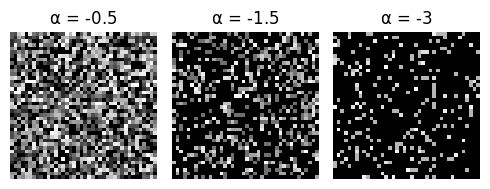
\includegraphics[height=4.5cm]{Images/ex_GI0.png}
    \caption{Tres imágenes generadas a partir de la distribución \( \mathcal{G}_I^0 \), con $L=\gamma=1$, y distintos valores de $\alpha$.}
    \label{fig:distintos_alphas}
\end{figure}

\subsection{Diseño del dataset}

Generamos imágenes partidas en cuadrantes, donde cada uno tiene un valor diferente de $\alpha$. Diseñamos una función que crea imágenes de este tipo, donde se toma como \emph{input} la cantidad de cuadrantes y la cantidad de píxeles del lado de los cuadrantes. En la figura \ref{fig:cuadrantes} se muestran algunos ejemplos. Los valores de $\alpha$ de donde muestreamos son: (-1.5, -2, -3, -5, -6, -8, -10, -20).

\begin{figure}[htbp]
    \centering
    \begin{subfigure}[b]{0.48\textwidth}
        \centering
        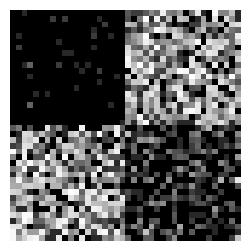
\includegraphics[height=5cm]{Images/cuadrantes1.png}
        \caption{4 cuadrantes}
    \end{subfigure}
    \hfill
    \begin{subfigure}[b]{0.48\textwidth}
        \centering
        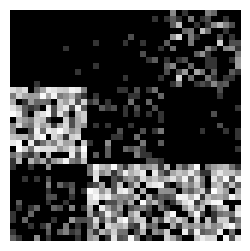
\includegraphics[height=5cm]{Images/cuadrantes2.png}
        \caption{9 cuadrantes}
    \end{subfigure}
    \caption{Ejemplos de imágenes partidas en cuadrantes, con distintos valores de $\alpha$ en cada uno. Todas con $L=\gamma=1$.}
    \label{fig:cuadrantes}
\end{figure}

Para la generación de datasets completos, elegimos el tipo de partición que se va a utilizar, y se generan múltiples imágenes en donde cada una, en cada cuadrante, tiene un valor de $\alpha$ seleccionado al azar. También contemplamos la posibilidad de crear datasets mixtos, es decir, con distintas particiones, aunque siempre con el mismo tamaño de imagen. Esto es con la intención de que el modelo no aprenda los bordes de los cuadrantes, sino que sepa generalizar.

Es importante destacar que no solo podemos generar las imágenes con distribución \( \mathcal{G}_I^0 \), sino que también podemos hacer las imágenes con distribución $\Gamma$ y $\Gamma^{-1}$ que componen a la primera. Es decir que podemos construir las imágenes correspondientes a $z$, $x$ e $y$ de la ecuación \ref{eq:zxy}. Recordemos que estas son la imagen ruidosa, la imagen limpia, y el ruido \emph{speckle} respectivamente. La figura \ref{fig:cuadrantes_xyz} muestra un ejemplo de estas tres componentes. Es interesante notar que en la figura \ref{subfig:cuadrantes_y} (ruido $speckle$) no se distinguen los cuadrantes. Esto es porque su distribución no depende de $\alpha$, como se ve en la ecuación \ref{eq:ruido_speckle}. Y como ya mencionamos, $\alpha$ es el único parámetro que estamos variando.

\begin{figure}[htbp]
    \centering
    \begin{subfigure}[b]{0.27\textwidth}
        \centering
        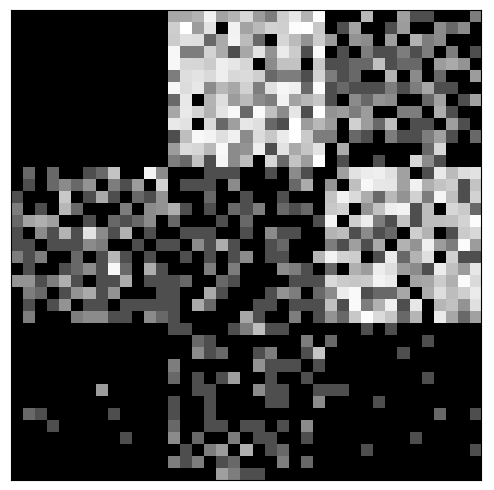
\includegraphics[height=5cm]{Images/cuadrantes_x.png}
        \caption{$x$: $\Gamma^{-1}$.}
        \label{subfig:cuadrantes_x}
    \end{subfigure}
    \hfill
    \begin{subfigure}[b]{0.27\textwidth}
        \centering
        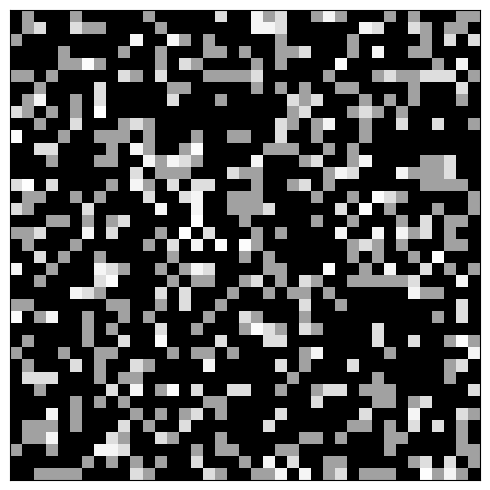
\includegraphics[height=5cm]{Images/cuadrantes_y.png}
        \caption{$y$: $\Gamma$}
        \label{subfig:cuadrantes_y}
    \end{subfigure}
    \hfill
    \begin{subfigure}[b]{0.27\textwidth}
        \centering
        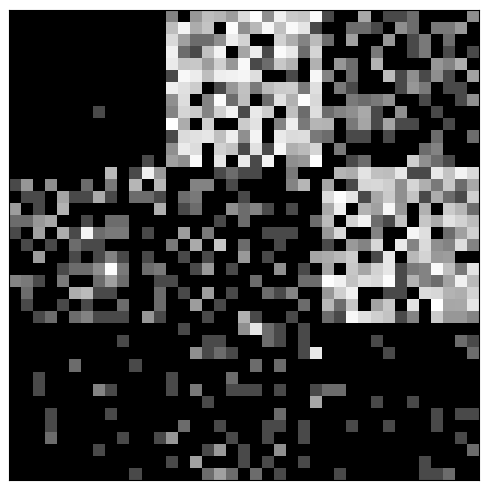
\includegraphics[height=5cm]{Images/cuadrantes_z.png}
        \caption{$z$: \( \mathcal{G}_I^0 \)}
        \label{subfig:cuadrantes_z}
    \end{subfigure}
    \caption{Ejemplo de tres imágenes, de 9 cuadrantes cada una, generadas artificialmente. (a) tiene distribución $\Gamma^{-1}$ y corresponde al backscatter, es decir, la imagen sin ruido. (b) sigue una distribución $\Gamma$ que representa al ruido \emph{speckle}. (c) sigue la distribución \( \mathcal{G}_I^0 \) y se corresponde con la imagen ruidosa. (c) se obtiene multiplicando, pixel a pixel, (a) con (b).}
    \label{fig:cuadrantes_xyz}
\end{figure}

\section{Redes neuronales multicapa y autoencoders}

\subsection{Redes neuronales multicapa (MLP)}

Las redes neuronales multicapa ($Multilayer Perceptron$, MLP) son arquitecturas de aprendizaje profundo compuestas por múltiples capas de neuronas artificiales interconectadas. Una MLP típica consta de una capa de entrada, una o más capas ocultas y una capa de salida. Cada neurona en una capa está conectada a todas las neuronas de la capa siguiente, formando una estructura completamente conectada (densa).

La operación fundamental en una MLP es la transformación lineal seguida de una función de activación no lineal. Para una capa $l$, la salida se calcula como:

\begin{equation}
\mathbf{h}^{(l)} = f(\mathbf{z}^{(l)}) = f(\mathbf{W}^{(l)}\mathbf{h}^{(l-1)} + \mathbf{b}^{(l)})
\end{equation}

donde $\mathbf{W}^{(l)}$ es la matriz de pesos, $\mathbf{b}^{(l)}$ es el vector de sesgos, y $f$ es la función de activación.

\subsection{Autoencoders}

Los autoencoders son un tipo particular de red neuronal que aprenden representaciones comprimidas de los datos de entrada. Constan de dos partes principales: un \textit{encoder} que comprime la entrada en una representación latente de menor dimensionalidad, y un \textit{decoder} que reconstruye la entrada original a partir de esta representación latente.

\begin{equation}
\mathbf{z} = f_{\text{encoder}}(\mathbf{x}), \quad \hat{\mathbf{x}} = f_{\text{decoder}}(\mathbf{z})
\end{equation}

Los autoencoders pueden verse como MLP especializadas donde la arquitectura está constraintida a tener una capa intermedia (cuello de botella) de menor dimensionalidad que fuerza al modelo a aprender características representativas de los datos.

\subsection{Extensión a datos bidimensionales: enfoque convolucional}

Tanto las MLP como los autoencoders pueden extenderse para procesar datos bidimensionales, como imágenes, mediante la incorporación de capas convolucionales. A diferencia de las capas densas que procesan la entrada completa mediante una transformación lineal global, las capas convolucionales aplican filtros de ventana que se deslizan sobre regiones locales de la imagen.

Este enfoque convolucional presenta varias ventajas significativas:
\begin{itemize}
    \item Preservación de información espacial: Al procesar pequeñas regiones de la imagen, se mantienen las relaciones espaciales entre píxeles.
    \item Invariancia ante traslaciones: Los filtros aprenden características independientemente de su posición en la imagen.
    \item Jerarquía de características: Las capas iniciales detectan patrones simples (bordes, texturas), mientras que capas más profundas combinan estas primeras para formar características más complejas.
\end{itemize}

En una capa convolucional, cada filtro procesa una pequeña ventana de la imagen de entrada (por ejemplo, 3×3 o 5×5 píxeles) y produce un valor de activación para el píxel correspondiente en el mapa de características de salida. Este proceso se repite para todas las posiciones espaciales, generando un mapa de características que preserva la estructura espacial de la entrada mientras extrae características relevantes.

Por supuesto que los autoencoders también pueden implementarse de forma convolucional. En este paradigma, el encoder utiliza capas convolucionales para comprimir progresivamente la representación de la imagen, mientras que el decoder emplea capas para reconstruir la entrada original a partir de la representación latente, manteniendo así las ventajas de preservación de la información espacial e invariancia traslacional propias de las convoluciones.

\subsection{Parámetros de las redes neuronales}\label{sec:params_red}

A continuación listamos los parámetros que definen a una red neuronal, y explicamos en qué consiste cada uno de ellos.

\titulito{Épocas y tamaño de \emph{batch}}
Una época corresponde a un paso completo del conjunto de datos de entrenamiento a través de la red. El número de épocas determina cuántas veces el algoritmo aprenderá del conjunto de datos completo.  El tamaño de lote (\emph{batch size}) define el número de muestras que se procesan antes de actualizar los parámetros del modelo, lo que se realiza comparando la salida generada con la salida esperada para calcular el error y ajustar los pesos. Además afecta la estabilidad y velocidad del entrenamiento.

\titulito{Funciones de activación}

Las funciones de activación son componentes que, recibiendo como entrada la suma ponderada de las neuronas de la capa anterior, transforman este valor para decidir si una neurona debe activarse o no. Al introducir no linealidad a la salida de cada capa, permiten que la red aprenda patrones complejos. Veamos ahora las funciones de activación que se usarán en este trabajo:

\begin{itemize}

    \item ReLU (\emph{Rectified Linear Unit}): Devuelve el valor de entrada si es positivo, y cero en caso contrario.
    \begin{equation}
        f(x) = \text{max}(0, x)
    \end{equation}
    
    \item \emph{Leaky} ReLU: Es igual a la función ReLU pero para el caso de $x<0$ devuelve un pequeño valor. Esto es para evitar anular completamente algunas neuronas.
    \begin{equation}
    f(x) = 
        \begin{cases}
        x & \text{si } x \geq 0, \\
        0.01x & \text{si } x < 0
        \end{cases}
    \end{equation}

    \item ELU (\emph{Exponential Linear Unit)}: Devuelve el valor de entrada si es positivo, y para valores negativos devuelve una exponencial suavizada que converge a un valor $\alpha$ negativo, reduciendo el problema de neuronas anuladas y mejorando la convergencia. Además es completamente derivable.
    \begin{equation}
    f(x) = 
        \begin{cases}
        x & \text{si } x \geq 0, \\
        \alpha(e^x - 1) & \text{si } x < 0
        \end{cases}
    \end{equation}
    
    \item Sigmoidea: Transforma cualquier valor de entrada en un rango entre 0 y 1, lo que permite interpretar su salida como una probabilidad, siendo ampliamente utilizada en problemas de clasificación binaria.
    \begin{equation}
        \sigma(x) = \frac{1}{1 + e^{-x}}
    \end{equation}
    
    \item Tangente hiperbólica: Transforma cualquier valor de entrada en un rango entre -1 y 1, centrando la salida en cero, lo que suele mejorar la convergencia en redes neuronales en comparación con la función sigmoidea.
    \begin{equation}
        \tanh(x) = \frac{e^x - e^{-x}}{e^x + e^{-x}}
    \end{equation}

\end{itemize}

\titulito{Función de pérdida}
La función de pérdida (también llamada función de costo) es una métrica fundamental que cuantifica cuán equivocadas están las predicciones del modelo comparándolas con los valores reales. Actúa como una guía durante el entrenamiento, calculando el error para cada ejemplo y proporcionando una medida única que el algoritmo de optimización busca minimizar. A través de un proceso iterativo, los parámetros del modelo se ajustan progresivamente utilizando el algoritmo de descenso por gradiente, el cual minimiza la función de pérdida actualizando dichos parámetros en la dirección opuesta a su gradiente, mejorando así la precisión y el rendimiento del modelo. En esencia, la función de pérdida define el objetivo que el modelo debe aprender para resolver una tarea específica.

Existen diversas funciones de pérdidas, pero en el presente trabajo usaremos el error cuadrático medio (MSE por sus siglas en inglés), definido como:

\begin{equation}
\text{MSE} = \frac{1}{n} \sum_{i=1}^{n} (y_i - \hat{y}_i)^2
\end{equation}
donde $y_i$ es el \emph{output} esperado y $\hat{y}_i$ es el obtenido, mientras que $n$ es la cantidad de ejemplos sobre los cuales el modelo aprende dentro de una iteración (tamaño de \emph{batch}).

\titulito{Learning rate y scheduler}

El \emph{learning rate} o tasa de aprendizaje ($lr$) es un hiperparámetro crítico que controla el tamaño del paso que se realiza en cada actualización de los parámetros del modelo durante el proceso de optimización. Un valor demasiado alto puede causar inestabilidad y divergencia, mientras que un valor demasiado bajo puede ralentizar extremadamente la convergencia o quedar atrapado en mínimos locales. Para abordar este equilibrio, se utilizan \emph{schedulers} o programadores de learning rate, que adaptan dinámicamente el valor de $lr$ durante el entrenamiento según criterios predefinidos, como el número de épocas, el valor de la pérdida o métricas de rendimiento, con el objetivo de mejorar la convergencia y el rendimiento final del modelo. Definimos ahora los \emph{schedulers} que usaremos aquí:

\begin{itemize}
    \item \emph{StepLR} (slr): Reduce el $lr$ cada cierto número de épocas, por un factor específico. Ambos valores son parámetros que el usuario selecciona.
    
    \item \emph{ReduceLROnPlateau} (rlrop): Reduce el $lr$  por un factor específico cuando la función de pérdida no mejora durante una cantidad dada de épocas seguidas. Ambos valores son parámetros que el usuario selecciona.

    \item \emph{ExponentialLR} (elr): Reduce el $lr$ exponencialmente con un factor seleccionado por el usuario.
\end{itemize}

\titulito{Optimizadores}

La función del optimizador es actualizar iterativamente los parámetros del modelo (pesos y sesgos) con el objetivo de minimizar la función de pérdida. Utilizando el gradiente de esta función, el optimizador ajusta los parámetros en la dirección opuesta (descenso del gradiente), pero incorporando estrategias avanzadas para mejorar la eficiencia y estabilidad del proceso. El optimizador no solo decide cómo se actualizan los pesos, sino también cuánto se ajustan en cada iteración, equilibrando velocidad de convergencia y precisión final.

\begin{itemize}
    \item Descenso por gradiente estocástico (SGD): Actualiza los parámetros usando el gradiente del lote actual. Es simple y computacionalmente eficiente, pero puede ser lento en converger y oscilar alrededor del mínimo.
    \item Adam (\emph{Adaptive Moment Estimation}): Es un optimizador que combina dos conceptos clave: el momento y la adaptabilidad. El momento se refiere a la incorporación de una media móvil de los gradientes pasados, que actúa como inercia para suavizar las actualizaciones y evitar oscilaciones, permitiendo escapar de mínimos locales y avanzar de manera más estable hacia la solución óptima. La adaptabilidad consiste en ajustar la tasa de aprendizaje de cada parámetro individualmente, lo que normaliza las actualizaciones en dimensiones con gradientes de distinta magnitud. Todo esto permite al algoritmo de Adam converger de manera rápida y eficiente, incluso en problemas con ruido o curvas de pérdida complejas, haciéndolo uno de los optimizadores más populares en el aprendizaje profundo.
\end{itemize}

\subsection{Tipos de capas y cálculo de dimensiones}\label{sec:tipos_capas}

Procedemos a examinar las capas que constituyen a una red neuronal convolucional. Estas son los componentes esenciales que transforman progresivamente la representación de la imagen de entrada, modificando sus dimensiones y extrayendo características de complejidad incremental, lo que permite a la red aprender patrones complejos. El objetivo es describir los principios de operación de cada tipo de capa empleada en este trabajo, junto con la metodología para calcular las dimensiones de salida resultantes tras cada transformación.

\titulito{Capa densa}

La capa densa o \emph{fully connected} es un tipo de capa en la que cada neurona está conectada a todas las de la capa anterior. Funciona realizando una combinación lineal de las características de entrada. A este tipo de capa hay que indicarle la cantidad de neuronas a las cuales se quiere proyectar las neuronas de la capa anterior. No hay ninguna restricción sobre este valor, más allá de que sea un entero positivo.

\titulito{Capa de convolución}

La capa convolucional es el núcleo fundamental de una red neuronal convolucional. Su operación consiste en aplicar un conjunto de filtros o \emph{kernels} (matrices de pesos ajustables) que se deslizan sobre la imagen de entrada o los mapas de características de la capa, generando imágenes de menor dimensión. Este proceso de convolución permite detectar patrones locales, como bordes, texturas y formas. Cada filtro genera un mapa de características diferente, capturando así tipos específicos de atributos visuales. La profundidad de la capa de salida (número de mapas de características) está determinada por la cantidad de filtros utilizados. Veamos los parámetros relevantes para este tipo de capa:
\begin{itemize}
    \item Canales de salida (filtros): Determina cuántos filtros diferentes aplicará la capa convolucional. Aunque es una visión simplificada del proceso real, puede pensarse que cada filtro aprenderá a detectar un patrón diferente (entre otros).
    
    \item Tamaño de ventana o \emph{kernel}: Define el tamaño de la ventana que se desliza sobre la imagen para realizar la convolución. Por ejemplo, si este valor es $5$, la ventana será de $5\times 5$ píxeles.
    
    \item \emph{Stride}: Determina cuántos píxeles saltea el \emph{kernel} al deslizarse sobre la imagen. Por ejemplo, un \emph{stride} de $1$ hace que la ventana se mueva pixel por pixel. En cambio, si el valor es $2$, salta de 2 en 2 píxeles, reduciendo las dimensiones espaciales a la mitad.
    
    \item \emph{Padding}: Añade píxeles alrededor de la imagen antes de aplicar la convolución, para controlar qué sucede en los bordes, cuando el \emph{kernel} sobresale de la imagen. Si el \emph{padding} es $0$, la imagen resultante se reduce porque se impide que el \emph{kernel} sobresalga. Si en cambio su valor es $1$, añade $1$ píxel de relleno en todos los bordes. Por defecto los píxeles adicionales tienen valor $0$, pero eso también puede cambiarse. Por último, se puede tomar valores de \emph{padding} distintos en la dirección vertical y la horizontal.
\end{itemize}

Veamos a continuación cómo se determina la dimensión de la imagen de salida de una capa de convolución. Llamemos \emph{Output Size} al tamaño de salida, ya sea el ancho o el alto. \emph{Input Size}, por su parte, es el tamaño de entrada. Y el \emph{Kernel Size} es el tamaño de la ventana. Entonces:
\begin{equation}
    \text{\emph{Output Size}} = \frac{\text{\emph{Input Size}} + 2 \cdot \text{\emph{Padding}} - \text{\emph{Kernel Size}}}{\text{\emph{Stride}}} + 1
\end{equation}
Y además, el número de canales de la salida es igual a la cantidad de filtros. Por otro lado, el requisito para que la convolución sea válida es el siguiente:
\begin{equation}
    \text{\emph{Input Size}} \geq (\text{\emph{Kernel Size}} - 2 \cdot \text{\emph{Padding}} - 1) \cdot \text{\emph{Stride}} + 1
\end{equation}

\titulito{Capa de convolución traspuesta o deconvolución}
Este tipo de capa realiza la operación inversa a la convolución. Entonces, en lugar de disminuir el tamaño de las imágenes, las agranda. Tiene los mismos parámetros salvo que se agrega el \emph{output padding}. Dada la naturaleza de la operación de convolución traspuesta, para un mismo tamaño de entrada, \emph{kernel}, \emph{stride} y \emph{padding}, pueden existir múltiples tamaños de salida posibles que sean matemáticamente correctos. El \emph{output padding} es un pequeño \emph{padding} adicional (generalmente de 0 o 1) que se aplica a la salida de la operación para resolver esta ambigüedad y especificar de manera unívoca la forma final. La dimensión de salida se determina con la siguiente fórmula:
\begin{equation}
\begin{split}
    \emph{\text{Output Size}} = &\, (\emph{\text{Input Size}} - 1) \cdot \emph{\text{Stride}} - 2 \cdot \emph{\text{Padding}} \\
                         & + \emph{\text{Kernel Size}} + \emph{\text{Output Padding}}
\end{split}
\end{equation}
Nuevamente, el número de canales de la salida es igual a la cantidad de filtros. Y la validez de la deconvolución está dada por:
\begin{equation}
    \emph{\text{Input Size}} \geq \frac{1 + 2\cdot\emph{\text{Padding}} - \emph{\text{Kernel Size}} - \emph{\text{Output Padding}}}{\emph{\text{Stride}}} + 1
\end{equation}

\titulito{Capa \emph{max-pooling}}
El max pooling es una operación que reduce el tamaño de la imagen conservando la información más importante. Funciona dividiendo la entrada en pequeñas regiones o ventanas (de tamaño dado por el \emph{kernel size}) y seleccionando solo el valor máximo de cada región. Así, se reduce la dimensionalidad, se hace la representación más manejable y se ayuda a que el modelo sea más robusto a pequeñas variaciones en la posición de los elementos. La salida se calcula de la siguiente manera:
\begin{equation}
    \emph{\text{Output Size}} = \frac{\emph{\text{Input Size}} + 2 \cdot \emph{\text{Padding}} - (\emph{\text{Kernel Size}} - 1) - 1}{\emph{\text{Stride}}} + 1
\end{equation}
Esta operación se realiza independientemente para cada canal de la imagen, con lo cual la cantidad de canales totales no varía. Y para que el \emph{max-pooling} sea válido debe cumplirse que:
\begin{equation}
    \emph{\text{Input Size}} \geq (\emph{\text{Kernel Size}} - 2\cdot \emph{\text{Padding}} - 1) \cdot \emph{\text{Stride}} + 1
\end{equation}

\titulito{Capa \emph{upsample}}
Mientras que la capa de \emph{max-pooling} reduce el tamaño de los datos (submuestreo), la capa \emph{upsample} aumenta el tamaño. Lo que hace es replicar o interpolar los valores existentes para llenar el nuevo espacio. Los métodos más comunes son el de vecinos más cercanos, donde simplemente copia el valor de cada píxel en las nuevas posiciones adyacentes, y el de interpolación bilineal, en donde se calcula un promedio ponderado de los píxeles circundantes para generar valores nuevos y más suaves. A la operación de \emph{upsample} únicamente hay que indicarle el factor por el cual se quiere agrandar la imagen.

\titulito{Capa \emph{flatten}}
La capa \emph{flatten} o de aplanamiento actúa como un puente entre las capas convolucionales o de \emph{pooling} (que procesan datos multidimensionales, como matrices 2D o 3D) y las capas densas (que requieren datos en formato unidimensional). Su función es tomar el tensor de entrada y "aplanarlo". Por ejemplo, si la entrada es un volumen de dimensiones (\emph{Input Height}, \emph{Input Width}, \emph{Input channels}), la capa \emph{flatten} lo convierte en un vector de tamaño:
\begin{equation}
    \emph{Output Dim.} = \emph{Input Height} \cdot \emph{Input Width} \cdot \emph{Input channels}
\end{equation}
Esto permite que la información espacial aprendida por las convoluciones sea interpretada por las capas densas.

\titulito{Capa \emph{unflatten}}
La capa \emph{unflatten} o de des-aplanamiento realiza la operación inversa a la capa \emph{flatten}. Toma un vector unidimensional y lo transforma en una estructura multidimensional. Actúa como un puente que permite traducir la información abstracta y compacta de las capas densas de vuelta a un formato de grilla, que luego puede ser procesado por capas convolucionales para generar una salida estructurada, como una nueva imagen. Solo es necesario que el producto entre las dimensiones de salida que le pedimos a la capa \emph{unflatten}, es decir (\emph{Output Height}, \emph{Output Width}, \emph{Output channels}), sea igual a la dimensión de entrada:
\begin{equation}
    \emph{Output Height} \cdot \emph{Output Width} \cdot \emph{Output channels} = \emph{Input Dim.}
\end{equation}

\vspace{1cm}

Todas las capas que presentamos aqui permiten construir arquitecturas complejas como los autoencoders convolucionales, donde el encoder típicamente utiliza capas convolucionales y de \emph{pooling}, mientras que el decoder emplea capas deconvolucionales y de \emph{upsampling} para reconstruir la entrada original.

\section{Desarrollo y entrenamiento de modelos}

El algoritmo que elegimos para la limpieza de imágenes SAR es un autoencoder convolucional. En este tipo de red neuronal, a diferencia de las tradicionales, la arquitectura de capas convolucionales le permite aprender patrones jerárquicos y locales, lo que resulta crucial para la preservación de la configuración de las imágenes. En cuanto a la estructura de autoencoder, esta elección se basa en la capacidad del mismo para comprimir y reconstruir datos permitiendo una limpieza efectiva sin perder información crítica. La expectativa es que en la capa interna, la más pequeña de todas, la red aprenda a codificar la imagen limpia y descarte el ruido.

El entrenamiento está basado en las imágenes artificiales que generamos de la forma expuesta anteriormente. El \emph{input} de la red es la imagen ruidosa, y el \emph{output} se compara contra la imagen limpia, la cual representa el \emph{target}. Esta es la principal diferencia con los autoencoder típicos, en donde el \emph{target} es igual al \emph{input}. Si miramos la figura \ref{fig:cuadrantes_xyz} por ejemplo, buscamos que la red nos devuelva \ref{subfig:cuadrantes_x} a partir de \ref{subfig:cuadrantes_z}.

Para generar un primer \emph{score} de testeo que nos permita comparar todas las arquitecturas que vamos a probar, creamos un conjunto de $1000$ imágenes, de la misma forma que construimos las imágenes de entrenamiento, para evaluar el modelo ya entrenado sobre el mismo. Para comparar usamos el error cuadrático medio entre la salida real de la red y la salida esperada. Esta es la misma métrica utilizada durante el entrenamiento. Luego se toma el error promedio entre las $1000$ imágenes.

\subsection{Arquitecturas}

Como parte del trabajo desarrollamos un framework de entrenamiento, que utiliza archivos de configuración para permitir una rápida experimentación con diversas arquitecturas de redes neuronales, sin la necesidad de modificar el código. Estos archivos permiten cambiar, por ejemplo, todos los parámetros explicados en \ref{sec:params_red} y \ref{sec:tipos_capas} en un mismo lugar, de forma centralizada. Y adicionalmente el código diseñado realiza los chequeos descritos en \ref{sec:tipos_capas} para asegurarse que las arquitecturas de los archivos de configuración sean válidas.

De esta manera probamos un total de $25$ arquitecturas. Enumeramos a continuación algunos de los parámetros principales que variamos: las imágenes usadas, el tipo de capa (convolución, deconvolución, $flatten$, $unflatten$, $max$-$pool$, $upsample$, densa), funciones de activación (ReLU, $Leaky$ ReLU, sigmoidea, tangente hiperbólica, ELU) y el optimizador (Adam, descenso por gradiente estocástico). A modo de ejemplo mostramos una de las arquitecturas probadas más en detalle, junto con su correspondiente error de test:

\begin{itemize}
    \setlength{\itemsep}{0pt}
    \item[-] \textbf{Imágenes:} $100,000$ imágenes $50\times 50$ de las cuales el 55\% tienen 4 particiones y el 45\% tienen una única partición.
    \item[-] \textbf{Épocas:} 500
    \item[-] \textbf{Batch size:} 64
    \item[-] \textbf{Capas encoder:}
            \begin{itemize}
            \setlength{\itemsep}{0pt}
                \item Capa de convolución bidimensional que transforma la imagen de $50\times 50$ de un solo canal (blanco y negro) en una de $25\times 25$ de $16$ canales. Filtros de $3\times 3$, \textit{padding} de $1$ y \textit{stride} de $2$. Función de activación ReLU.
                \item Capa de tipo \textit{flatten} que aplana la imagen a un vector de dimensión $10,000$. Notar que  que $25*25*16=10,000$.
                \item Capa densa que reduce el vector a la capa final de encoding, de dimensión $32$. Función de activación ReLU.
            \end{itemize}
    \item[-] \textbf{Capas decoder:}
            \begin{itemize}
            \setlength{\itemsep}{0pt}
                \item Capa densa que aumenta el vector a uno de dimensión $10,000$. Función de activación ReLU.
                \item Capa de tipo \textit{unflatten} que transforma el vector en una imagen de $25\times 25$ de $16$ canales.
                \item Capa de convolución bidimensional traspuesta que transforma la imagen en una de igual dimensión que la original, es decir de $50\times 50$ y $16$ canales. Filtros de $2\times 2$, \textit{padding} de $0$ y \textit{stride} de $2$. Función de activación sigmoidea.
            \end{itemize}
    \item[-] \textbf{LR y Scheduler:} LR inicial de $0.001$ adaptado mediante ELR (exponential learning rate scheduler) que disminuye el LR exponencialmente.
    \item[-] \textbf{Optimizador y función de pérdida:} Adam y MSE (error cuadrático medio).
\end{itemize}

Este mismo autoencoder está esquematizado en la figura \ref{fig:esquema_red}. Allí se puede apreciar la naturaleza simétrica de esta red, y como en la capa interna se comprime la información contenida en la imagen. También podemos ver que la primera mitad corresponde al \textit{encoder}, encargado de codificar la información en un espacio de dimensión menor, mientras que la segunda mitad se conoce como \textit{decoder}, el cual intenta reconstruir una imagen de tamaño original.

\begin{figure}[htbp]
    \centering
    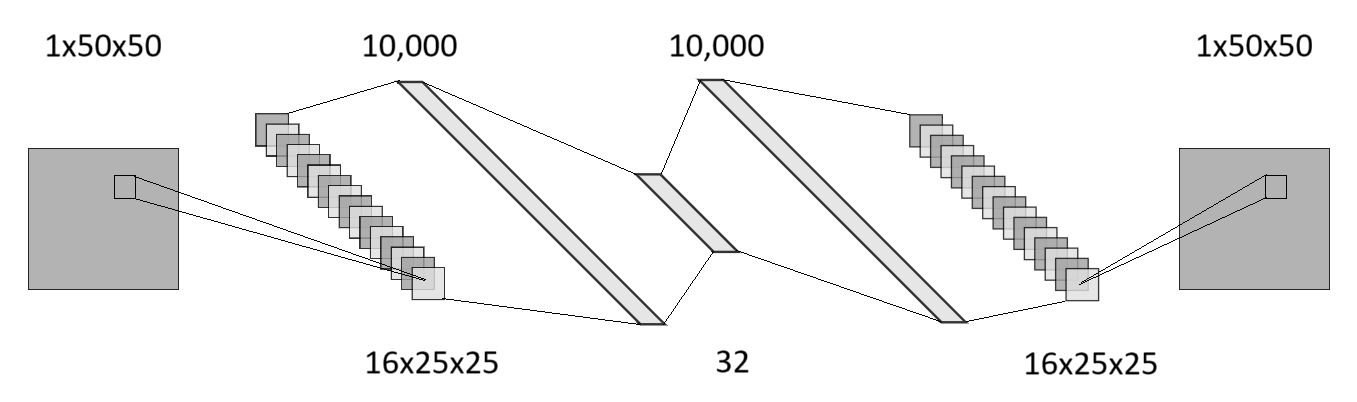
\includegraphics[height=4.5cm]{Images/red.png}
    \caption{Esquema de un autoencoder en donde la imagen ($50\times 50$ en blanco y negro) se reduce mediante una convolución a $16$ canales de $25\times 25$. Una capa \textit{flatten} la convierte en un vector de $10,000$ dimensiones, que se comprime a $32$ mediante una capa densa. El proceso se invierte para construir una imagen de $50\times 50$.}
    \label{fig:esquema_red}
\end{figure}

\section{Medición de la calidad del filtro}

Además del error de testeo existen otros métodos que permiten medir la calidad del filtro, es decir, qué tan buena fue la eliminación del ruido. Uno de ellos es pasar imágenes SAR reales por el autoencoder ya entrenado y verificar cómo es la salida. Sin embargo, este es solamente un método visual. Dado que no poseemos las imágenes limpias, no podemos cuantificar la bondad del filtro con esta técnica.

Otros métodos que sí nos permiten medir el desempeño del modelo son los que se basan en las propiedades estadísticas de las imágenes y de las distribuciones subyacentes. A continuación las describimos en mayor detalle.

\subsection{Métodos estadísticos}

Recordemos que, según el modelo multiplicativo condensado en la ecuación \ref{eq:zxy}, la imagen SAR ($z$) se puede obtener como el producto entre la imagen limpia ($x$) y el ruido \emph{speckle} ($y$). Esto implica que si tomamos el ratio punto a punto entre la imagen original y la filtrada, esperaríamos obtener una imagen sin ninguna estructura ni patrón geométrico presente, simplemente puro ruido \emph{speckle}. A este ratio lo denominamos $I = z/x$, y es lo que queremos que sea similar a $y$. Este es el principio en el cual se basan los métodos estadísticos que explicaremos.

\titulito{Método de primer orden}
Un mayor número de \emph{looks} genera una imagen menos ruidosa, con lo cual esperamos que un buen filtro aumente el número equivalente de \emph{looks}. Y además no debería cambiar la media del valor de la imagen dentro de una zona homogénea ($\mu$). Si al desvío estándar dentro de esa misma zona lo denominamos $\sigma$, entonces $\text{ENL} = \mu^2 / \sigma^2$. En una imagen suave, es decir con un $\text{ENL}$ grande, el desvío se vuelve insignificante respecto de la media. Seleccionando N zonas homogéneas dentro de nuestras imágenes, podemos cuantificar la variación del número equivalente de looks entre la imagen ruidosa y la filtrada en la zona $i$ como:
\begin{equation}\label{eq:renl}
    r_{\text{ENL}}(i) = \frac{\big|\text{ENL}_z(i) - \text{ENL}_I(i)\big|}{\text{ENL}_z(i)}
\end{equation}
donde el índice $i$ va entre 1 y N. Y recordemos que $z$ se refiere a la imagen original, mientras que $I$ es el ratio entre $z$ y la imagen filtrada. Luego, como la media debería permanecer invariante, esperaríamos que la media de $I$ sea cercana a $1$. Podemos medir esto de la siguiente manera:
\begin{equation}\label{eq:rmu}
    r_{\mu}(i) = \big|1-\mu_I(i)\big|
\end{equation}
donde $\mu_I(i)$ es la media sobre la imagen ratio en la zona $i$. Sumando las cantidades dadas por \ref{eq:renl} y \ref{eq:rmu} obtenemos el estadístico de primer orden:
\begin{equation}
    r_{\text{ENL},\mu} = \frac{1}{2N}\sum_{i=1}^{N} \big( r_{\text{ENL}}(i) + r_{\mu}(i) \big)
\end{equation}
El valor de $r_{\text{ENL},\mu}$ siempre es positivo, e idealmente valdría $0$.

Típicamente trabajaremos con imágenes de tamaño $50\times 50$ y $4$ o $5$ zonas de $10\times 10$. También debemos asegurarnos que esas zonas sean homogéneas. Para eso las elegimos sin cruzarnos de cuadrante, y solo en aquellos cuadrantes en donde $\alpha\in(-\infty,-6)$.

\titulito{Método de segundo orden}
Como mencionamos, un buen filtro debería producir una imagen ratio $I$ sin contenido geométrico. Una forma de medir esto es a través del coeficiente de homogeneidad $h$ de las matrices de co-ocurrencia de Haralik. Definamos ahora qué significa esto.

Las matrices de Haralick, también conocidas como matrices de dependencia espacial de grises o GLCM por su siglas en inglés (\emph{Gray-Level Co-occurrence Matrices}), capturan las relaciones espaciales entre los píxeles de una imagen. Se construyen calculando con qué frecuencia un par de píxeles con valores de intensidad específicos ($i$, $j$) aparecen en la imagen separados por una distancia $d$ y una dirección $\theta$ específicas. En esencia, una GLCM es una matriz cuadrada donde cada elemento $p(i, j | d, \theta)$ representa la probabilidad de que dos píxeles adyacentes (según la distancia y ángulo definidos) tengan los valores de gris $i$ y $j$.

A partir de estas matrices se pueden calcular un conjunto de descriptores o características de Haralick, que son medidas estadísticas que cuantifican propiedades específicas de la textura, como el contraste, la uniformidad, la entropía o la correlación. El coeficiente de homogeneidad ($h$), también conocido en inglés como \emph{Inverse Difference Moment}, es precisamente uno de estos descriptores. Mide la uniformidad local de la imagen y qué tan cerca se distribuyen los elementos de la GLCM de su diagonal principal. Definimos $p(i,j)$ como el valor normalizado en la posición $(i, j)$ de la matriz de co-ocurrencia, cuya dimensión es $M\times M$ con $M$ igual al número de niveles de gris que tiene la imagen. Entonces, el coeficiente de homogeneidad se define de la siguiente forma:
\begin{equation}
    h = \sum_{i=1}^{M}\sum_{j=1}^{M}\frac{p(i,j)}{1+(i-j)^2}
\end{equation}
Para un filtro perfecto la densidad de probabilidad de $I$ es invariante ante permutaciones aleatorias, justamente porque la imagen ratio no debería tener estructuras. Por lo tanto el valor de $h$ tampoco debería variar en dichas circunstancias. Para medir esta variación definamos $h_0$ como el valor de $h$ sobre la imagen $I$ sin permutaciones, y $h_m$ al valor después de la permutación $m$-ésima, con $m$ entre $1$ y el número total de permutaciones $g$. Definimos entonces la variación porcentual entre ambas cantidades como:
\begin{equation}
    \delta_h = 100\Bigg| \frac{1}{h_0} \Bigg( h_0 - \frac{1}{g}\sum_{m=1}^{g} h_m \Bigg) \Bigg|
\end{equation}
A esto se lo conoce como el estadístico de segundo orden. Un $\delta_h$ más pequeño indica una menor cantidad de información geométrica y estructural en la imagen ratio, lo cual a su vez es evidencia de un mejor filtro. Cada una de las $g$ permutaciones las haremos al azar, evitando así cualquier sesgo que pudiéramos introducir.

Si sumamos ambos estadísiticos de la forma propuesta en \cite{gomez2017unassisted}, obtenemos una medida intregrada de la bondad del método de limpieza:
\begin{equation}
    \mathcal{M} = r_{\text{ENL},\mu} + \delta_h
\end{equation}
Esperamos que $\mathcal{M}$ sea lo más chico posible. Este valor se obtiene a partir de una única imagen. Si bien es presumible que $\mathcal{M}$ se mantendrá aproximadamente constante sobre todas las imágenes dado que son sintéticas, tomaremos el valor medio sobre todo el dataset de testeo y ese será el valor que reportaremos.

\subsection{Comparación con otros filtros}

Otra forma de mesurar el rendimiento del modelo entrenado es comparándolo con métodos alternativos. Por un lado se puede contrastar los estadísticos obtenidos con los de otros trabajos reportados en la literatura, como puede ser el de \cite{chan2022entropy}. Esta no es más que una comparación en orden de magnitud, ya que las imágenes usadas para evaluar no son las mismas. Por otro lado, la aplicación sobre nuestro dataset de métodos clásicos para el \emph{despeckling} permite una comparación directa del desempeño de ambos modelos. En este trabajo usaremos el filtro de Lee como punto de referencia para nuestro autoencoder.

El filtro de Lee \cite{lee1980digital} es un método clásico de filtrado no lineal ampliamente utilizado en el procesamiento de imágenes con ruido \emph{speckle}. Conceptualemente, opera bajo el principio de minimizar el error cuadrático medio dentro de una ventana local deslizante. El filtro calcula un promedio ponderado de los píxeles en una vecindad, donde el peso de cada píxel depende de las estadísticas locales de ruido y señal. Además ajusta el nivel de suavizado según el contraste local, es decir, suaviza mucho en áreas uniformes y conserva detalles en áreas con bordes o variación. Aunque algunas desventajas son que suele generar halos en las intersecciones de terrenos muy distintos como puede ser agua y mar, y que sus resultados dependen del tamaño de la ventana del filtro, el cual debe ser elegido manualmente.

\section{Entrenamiento con imágenes reales}

Una opción alternativa al entrenamiento con imágenes sintéticas, es usar imágenes reales. Pero como ya dijimos, no existen las imágenes SAR limpias que nos permitan entrenar un modelo de machine learning supervisado. Sin embargo, el trabajo presentado en \cite{vasquez2024labeled} muestra como consiguieron imágenes sin ruido \emph{speckle} promediando numerosas imágenes tomadas en el mismo lugar. Con este método generaron un dataset de pares de imágenes ruidosas y limpias, y las pusieron a disposición del público. Nuestro objetivo entonces es entrenar otros autoencoder utilizando esta base de datos.

El dataset en cuestión está compuesto por 1600 pares de imágenes de $512\times 512$, tomadas en zonas muy variadas, como agua, costanera, zonas rurales y urbanas. Un ejemplo se encuentra en la figura \ref{fig:dataset_sar}. Para poder entrenar al autoencoder libremente y no precisar tomar como input imágenes de $512$ píxeles de lado, diseñamos una función que permite cortar el dataset en imágenes más pequeñas. Una vez hecho esto dividimos el conjunto en entrenamiento y testeo, y lo usamos para entrenar el autoencoder intentando que genere la imagen limpia a partir de la ruidosa.

\begin{figure}[htbp]
    \centering
    \begin{subfigure}[b]{0.49\textwidth}
        \centering
        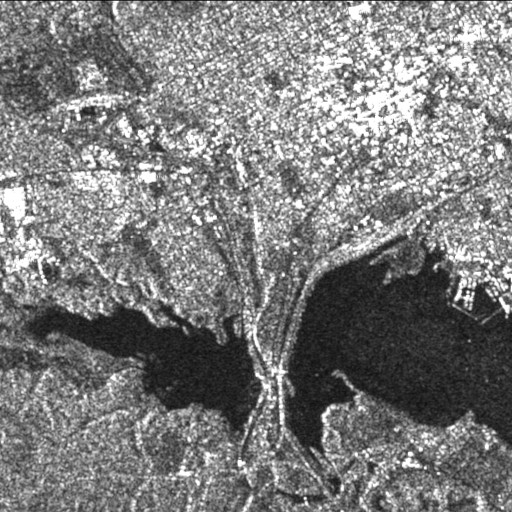
\includegraphics[height=7cm]{Images/noisy_ex.jpg}
        \caption{Imagen SAR original}
    \end{subfigure}
    \hfill
    \begin{subfigure}[b]{0.49\textwidth}
        \centering
        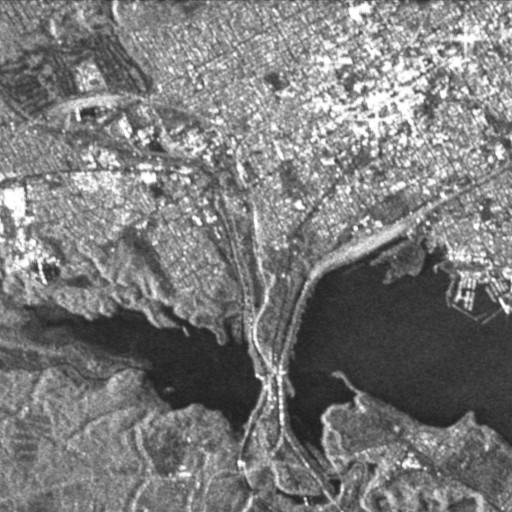
\includegraphics[height=7cm]{Images/clean_ex.jpg}
        \caption{Imagen SAR limpia}
    \end{subfigure}
    \caption{Ejemplo de imagen SAR y su contraparte sin ruido \emph{speckle} conseguida promediando varias imágenes del mismo sitio.}
    \label{fig:dataset_sar}
\end{figure}

En los autoencoders entrenados con imágenes reales no podemos evaluar el rendimiento usando los estadísticos de primer y segundo orden. Esto se debe a que para hacerlo sería necesario tomar zonas homogéneas de la imagen. En el caso de imágenes sintéticas es muy sencillo, ya que se reduce a observar el valor de $\alpha$. Pero para imágenes reales el proceso es significativamente más complicado, es por esto que solo evaluaremos el modelo mediante su error de testeo.